	\documentclass[a4paper]{article}
	
	\usepackage[portuguese]{babel}
	\usepackage[utf8]{inputenc}
	\usepackage{indentfirst}
	\usepackage{graphicx}
	\usepackage{verbatim}
	\usepackage{wrapfig, blindtext}
	\usepackage{listings}
	\usepackage{textcomp}
	\usepackage{color}
	\usepackage{xcolor}
	\usepackage[left=1in,right=1in,top=1in,bottom=.8in]{geometry}
	\usepackage{float}
	\usepackage{titlesec}
	\usepackage{csvtools}

\graphicspath{ {res/} }

	%%%%%%%%%%% CONFIGURATION OF CODE INPUT %%%%%%%%%%%%%%%%%%%%%%
\lstset{
  language=C,
  tabsize=4,
  captionpos=b,
  numbers=left,
  frame=single,
  breaklines=true,
  rulecolor=\color{black},
  title=Struct linkLayer,
  commentstyle=\color{codeGreen},
  backgroundcolor=\color{codeBackground},
  numberstyle=\color{gray},
  keywordstyle=\color{blue} \textbf,%otherkeywords={xdata},
  keywords=[2]{xdata},
  keywordstyle=[2]\color{red}\textbf,
  identifierstyle=\color{black},
  stringstyle=\color{red}\ttfamily,
  basicstyle = \ttfamily \color{black} \footnotesize,
  showstringspaces=false ,
}
%%%%%%%%%%%%%%%%%%%%%%%%%%%%%%%%%%%%%%%%%%%%%%%%%%

	\begin{document}
	

\definecolor{codeBackground}{RGB}{220, 220, 220}
\definecolor{codeGreen}{RGB}{0, 150, 0}
	\setlength{\textwidth}{16cm}
	\setlength{\textheight}{22cm}
	
	\title{\Huge\textbf{Lab 2}\linebreak\linebreak\linebreak
	\Large\textbf{Relatório Final}\linebreak\linebreak
	\linebreak\linebreak
	
\includegraphics[scale=0.1]{./res/feup-logo.png}\linebreak\linebreak
	\linebreak\linebreak
	\Large{Mestrado Integrado em Engenharia Informática e Computação} \linebreak\linebreak
	\Large{Redes de Computadores}\linebreak
		}
	

	\author{
	\textbf{Grupo 3:}\\
	Francisco Rodrigues - 201305627 \\
	João Nogueira - up201303882 \\
	Marta Lopes - 201208067 \\
	\linebreak\linebreak \\
	 \\ Faculdade de Engenharia da Universidade do Porto \\ Rua Roberto Frias, s\/n, 4200-465 Porto, Portugal \linebreak\linebreak\linebreak
	\linebreak\linebreak\vspace{1cm}}
	
	\maketitle
	\thispagestyle{empty}

	\newpage

	\tableofcontents	

	\newpage

	\section{Sumário}
	\normalsize

Este relatório tem como objetivo explicar o segundo projeto da Unidade Curricular de Redes de Computadores bem como analisar os resultados obtidos na realização das experiências especificadas no enunciado do mesmo.

	\section{Introdução}

	Este projeto encontra-se dividido em duas grandes partes. Em primeiro lugar, é-nos pedido que desenvolvamos uma aplicação de \textit{download} que proceda à transferência de um ficheiro e que implemente o protocolo \textit{FTP}. Em segundo lugar, é-nos pedido que configuremos e estudemos uma Rede de Computadores seguindo a estrutura das experiências abaixo enumeradas:

\begin{enumerate}

\item Configuração de um \textit{IP} de rede;
\item Configuração de duas Redes \textit{LAN} virtuais num \textit{switch};
\item Configuração de um \textit{router} em \textit{Linux};
\item Configuração de um \textit{router} comercial implementando \textit{NAT};
\item \textit{DNS};
\item Conexões \textit{TCP}.

\end{enumerate}

	\section{Parte 1 - Aplicação de download}

	Como referido anteriormente, a primeira parte deste tranalho consiste numa aplicação que transfere um ficheiro utilizando o protocolo \textit{FTP} descrito no ficheiro RFC959. Como método de \textit{input} é utilizada a sintaxe mostrada na figura abaixo como descrito no ficheiro RFC1738.

	\begin{figure}[H]
  	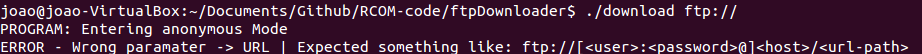
\includegraphics[width=\linewidth]{consoleScreenshot1.png}
  	\caption{Input}
  	\label{fig:input}
	\end{figure}

	A aplicação desenvolvida permite que seja feito um download em modo anónimo. Para tal basta não colocar os caracteres '@' e ':' e não colocar nome de utilizador e password. Neste caso a aplicação irá assumir o utilizador \textit{anonymous} e a palavra-passe vazia.

	\subsection{Arquitetura}

	A \textit{UrlStruct} é a estrutura definida respponsável por guardar a informação necessária que depende do \textit{input} do utilizador.

	\lstset{basicstyle=\ttfamily \color{black}\tiny, title=urlStruct}
	\lstinputlisting{./res/res1.c}
	\normalsize

	Ao correr o programa é chamada a função \textit{getUrlInfo} que é responsável por pegar na \textit{string} que o utilizador forneceu como argumento e interpretar toda a informação necessária.

	\lstset{basicstyle=\ttfamily \color{black}\tiny, title=Url Header}
	\lstinputlisting{../ftpDownloader/url.h}
	\normalsize

	Depois de interpretar a informação introduzida pelo utilizador, e após verificar que esta informação é válida é chamada a função \textit{startConection} responsável por ligar o cliente \textit{FTP} ao servidor através de um \textit{socket}. Com a ligação estabelecida é então necessário chamar função \textit{getControl}, responsável por enviar a informação necessária para o \textit{login} e por enviar o comando \textbf{\textit{PASV}}, o que vai permitir que haja comunicação em ambos os sentidos.

	\lstset{basicstyle=\ttfamily \color{black}\tiny, title=getControl}
	\lstinputlisting{./res/res2.c}
	\normalsize

	 É também feita uma nova conexão através da função \textit{startReceiverConection} para permitir a receção do ficheiro. pedido pelo utilizador. Por fim é enviado o comando \textbf{\textit{RETR}} e recebido o ficheiro a ser guardado. A função \textit{receiveFile} é responsável por enviar o comando, receber o ficheiro e escrevê-lo no disco.

	Terminada a receção do ficheiro resta apenas fechar os \textit{sockets} abertos e libertar a memória alocada para terminar o programa.

	As funções acima referidas e outras auxiliares estão definifdas abaixo, bem como nos anexos.

	\lstset{basicstyle=\ttfamily \color{black}\tiny, title=conection.h}
	\lstinputlisting{../ftpDownloader/conection.h}
	\normalsize
	
	Durante o desenvolvimento da aplicação foi implementado um modo de \textit{debug} que é ativo ao alterar a Macro \textit{DEBUG} de 0 para 1. Este modo faz com que haja mais impressões na consola, o que permite controlar com maior exatidão o modo como a aplicação está a funcionar.

	\lstset{basicstyle=\ttfamily \color{black}\tiny, title=Macros}
	\lstinputlisting{./res/res3.c}
	\normalsize

	\subsection{Resultados}

	Esta aplicação foi testada com diversos ficheiros, tanto em modo anónimo como em modo não anónimo. A transferência dos vários ficheiros foi verificada tendo sido o máximo ficheiro testado um ficheiro de vídeo com cerca de 200MB.

	Em caso de erro, para além da aplicação terminar é impresso na consola o erro em causa, de modo a que o utilizador tenha o máximo controlo possível sobre o sucedido.

	\section{Parte 2 - Configuração de Redes}
	
	\subsection{Configuração de um IP de rede}

	\begin{figure}[H]
	\begin{center}
  	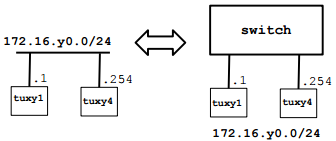
\includegraphics[width=0.45\linewidth]{exp1.png}
  	\caption{Experiment 1}
  	\label{fig:Experiment 1}
	\end{center}
	\end{figure}

	Esta primeira experiência tem como objetivo configurar duas máquinas numa só rede e compreender o seu funcionamento. Foram então configurados os dois computadores \textbf{tux41} e \textbf{tux44} para que estes assumissem os endereços de \textbf{IP} de \textbf{172.16.40.1} e \textbf{172.16.40.254}, respetivamente.

Para tal, utilizamos o comando \textbf{ifconfig}, atribuindo estes mesmos valores e ativando as portas \textbf{eth0} às quais foram ligados os cabos de rede.

Apos a configuração, através do comando \textbf{ping} verificou-se que existia a ligação entre as duas máquinas. Após esta verificação foram apagadas todas as entradas na tabela \textbf{ARP} através do comando \textbf{arp -d 'ip address'}. Por fim repetiu-se o comando \textbf{ping} registando o processo através do programa \textit{wireshark}.

	Analisando o \textit{log} do \textit{wireshark} da figura \ref{fig:Experiment 1 - log} nos Anexos, podemos verificar que, tendo apagado as entradas na tabela \textbf{ARP} é perguntado à rede qual o endereço \textbf{MAC} com um endereço de \textbf{IP} igual a \textbf{172.16.40.254}. Este computador responde com o seu endereço \textbf{MAC} e, a partir de aí, sempre que o primeiro faz um request \textbf{ICMP}, este é seguido de uma resposta do segundo. Verifica-se também que, como o endereço \textbf{MAC} do segundo se encontra na tabela \textbf{ARP} do primeiro, não é necessário haver mais nenhum \textbf{broadcast} como o da linha 5 do \textit{log} acima.

	\subsection{Configuração de duas redes \textit{LAN} virtuais num \textit{switch}}

	\begin{figure}[H]
	\begin{center}
  	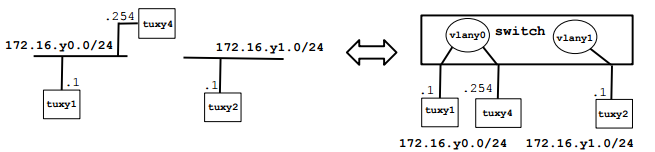
\includegraphics[width=0.8\linewidth]{exp2.png}
  	\caption{Experiment 2}
  	\label{fig:Experiment 2}
	\end{center}
	\end{figure}

	Esta experiência consiste na criação de duas \textit{vlan's} diferentes:

	\begin{itemize}
	\item \textit{VLAN 40} - \textit{172.16.40.0/24} -  à qual pertencem os computadores \textit{tux1} e \textit{tux4};
	\item \textit{VLAN 41} - \textit{172.16.41.0/24} -  à qual pertence o computador \textit{tux2}.
	\end{itemize}

	De notar que no final da configuração das máquinas e do \textit{switch} o computador \textit{tux2} deixará de ter acesso aos computadores que pertencem à rede \textit{VLAN 40}, à qual não pertence.

Para configurar os computadores da forma referida basta proceder do mesmo modo que se procedeu para a primeira experiência, mas desta vez fazê-lo no computador \textit{tux2} e atribuindo \textbf{172.16.41.1} como endereço de \textit{IP} (tendo em conta que os outros dois computadores continuam com a configuração da primeira experiência).

Para configurar o \textit{switch} acede-se à sua consola através da aplicação \textit{gkterm} e corre-se os comandos especificados em anexo.

	Estando os dois computadores na mesma rede, então, ao fazer \textbf{ping} do \textit{tux1} para o \textit{tux4}, não é enviado o pacote \textit{ARP} para saber o endereço \textit{MAC}, como se pode verificar na figura \ref{fig:Experiment 2 - Point 6}.

	Pode também verificar-se, na análise das figuras \ref{fig:Experiment 2 - Point 9 - tux1}, \ref{fig:Experiment 2 - Point 9 - tux2}, \ref{fig:Experiment 2 - Point 9 - tux4}, \ref{fig:Experiment 2 - Point 10 - tux1}, \ref{fig:Experiment 2 - Point 10 - tux2} e \ref{fig:Experiment 2 - Point 10 - tux4} que cada \textit{vlan} tem um \textit{broadcast domain} diferente, tendo em conta que o \textit{tux2} não detetou o pacote enviado, como tal, conclui-se que a configuração destas reder foi feita da forma correta pois verifica-se a falta de comunicação entre as redes, como foi referido no início desta experiência. Nas primeiras três figuras foi feito um \textit{broadcast} na \textit{vlan 41} enquanto que nas últimas três foi feito na \textit{vlan 41}.


	\subsection{Configuração de um \textit{router} em \textit{Linux}}

	\begin{figure}[H]
	\begin{center}
  	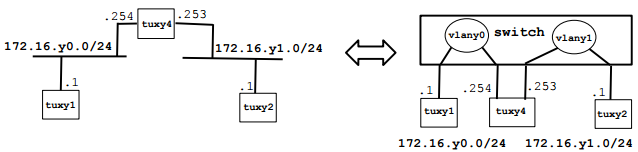
\includegraphics[width=0.8\linewidth]{exp3.png}
  	\caption{Experiment 3}
  	\label{fig:Experiment 3}
	\end{center}
	\end{figure}

	Esta experiência consiste na configuração do computador \textit{tux4} como \textit{router} por forma a ligar as duas \textit{vlan's} existentes:

	\begin{itemize}
	\item \textbf{172.16.40.0/24} - \textit{vlan 40};
	\item \textbf{172.16.41.0/24} - \textit{vlan 41}.
	\end{itemize}

	Em primeiro lugar ativa-se a porta \textit{eth1} do \textit{tux4} i liga-se ao \textit{switch}. Esta porta será a que será ligada à \textit{vlan 41}. Configura-se esta mesma porta com o endereço \textit{IP} \textbf{172.16.41.253/24}. Sendo este computadro aquele que pretendemos que sirva de \textit{router}, é necessário ativar o reencaminhamento de \textit{IP's} através do comando:

	\lstset{
   	language=[gnu] make,
   	keywordstyle=\color{teal}\textbf,
   	stringstyle=\color{blue},
   	identifierstyle=\itshape,
	 basicstyle = \ttfamily \color{black} \small,
	title=Shell Command
	}
	
	\begin{lstlisting}	
	echo 1 > /proc/sys/net/ipv4/ip_forward
	\end{lstlisting}

	Por fim, adicionou-se as rotas necessárias no \textit{tux1} e no \textit{tux2} por forma a que estes, através do \textit{tux4} pudessem aceder à rede a que não pertencem. Estas rotas forma adicionadas utilizando o comando:

	\begin{lstlisting}
	route add -net _ _
	\end{lstlisting}

	Como é possível analisar através da figura \ref{fig:Experiment 3 - tux1}, agora é possível a comunicação entre qualquer uma das três máquinas.

	\subsection{Configuração de um \textit{router} comercial implementando \textit{NAT}}

	\begin{figure}[H]
	\begin{center}
  	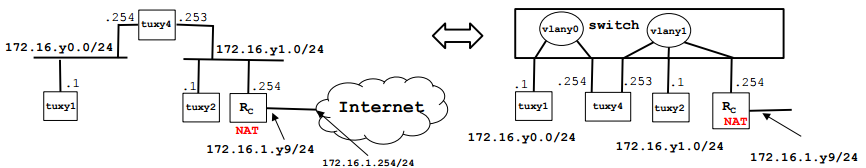
\includegraphics[width=0.8\linewidth]{exp4.png}
  	\caption{Experiment 4}
  	\label{fig:Experiment 4}
	\end{center}
	\end{figure}

	Esta experiência tem como objetivo a configuração do \textit{CISCO} dentro da rede 41 de forma a que tanto os computadores na \textit{vlan40} como na \textit{vlan41} tenham acesso à Internet.

	Para configurar o router, depois de fazer \textit{login} na linha de comandos corre-se o \textit{script} do Anexo 9. Os comandos referidos em anexo começam por configurar duas interfaces do \textit{router}, atribuindo corretamente as configurações \textit{NAT}. A configuração correta do \textit{NAT} é essencial pois a falta desta poderia resultar em falta de acesso à Internet em qualquer um dos computadores pois, como sabemos, \textit{NAT} tem a função de traduzir endereços, resultando neste caso na tradução do endereço de sub-rede de cada computador no endereço do \textit{router} comercial.
	
	Depois de permitir que os computadores das redes criadas tenham acesso, é configurada uma rota predefinida para o endereço da Internet. Da mesma forma é adicionada aos computadores a rota predefinida para o endereço \textbf{172.16.41.254}, endereço do \textit{router} comercial.

	Como é possível verificar na figura \ref{fig:Experiment 4 - tux1}, mesmo o computador da rede 10 tem acesso ao \textit{router} comercial.

	\subsection{\textit{DNS}}

	\begin{figure}[H]
	\begin{center}
  	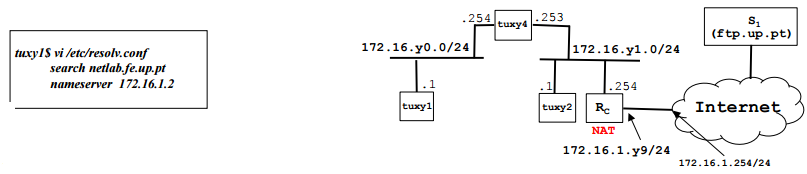
\includegraphics[width=0.8\linewidth]{exp5.png}
  	\caption{Experiment 5}
  	\label{fig:Experiment 5}
	\end{center}
	\end{figure}

	Esta experiência consiste apenas em adicionar um \textit{DNS}, como tal, basta colocar duas linhas no ficheiro \textbf{resolv.conf} situado no diretório \textbf{/etc} nos computadores com o sistema operativo em \textit{Linux}. Este ficheiro ficou então com as linhas abaixo:

	\lstset{
	title=resolf.conf
	}

	\begin{lstlisting}
	search lixa.netlab.fe.up.pt
	nameserver 172.16.1.1
	\end{lstlisting}

	Por fim foi testada a funcionalidade desta alteração acedendo, através do \textit{browser} a um \textit{website} o que, como podemos verificar na figura \ref{fig:Experiment 5 - tux1} se verificou sem problemas.

	\subsection{Conexões \textit{TCP}}

	\begin{figure}[H]
	\begin{center}
  	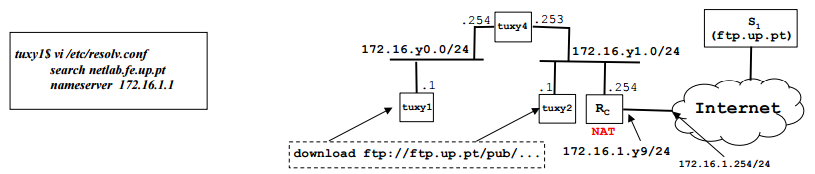
\includegraphics[width=0.8\linewidth]{exp6.png}
  	\caption{Experiment 6}
  	\label{fig:Experiment 6}
	\end{center}
	\end{figure}

	Esta experiência tinha como objetivo juntar as duas partes deste trabalho, pondo em prática a aplicação de \textit{download} desenvolvida na Parte 1 deste trabalho na rede cobfigurada ao longo destas experiências. A aplicação foi testada em modo anónimo e não anónimo, com ficheiros de imagem e de vídeo sendo que o ficheiro testado com maior tamanho tinha cerca de 200Mb. Foi também testada esta aplicação em simultâneo no \textit{tux1} e no \textit{tux2}, não tendo ocorrido qualquer tipo de problema na transferência do ficheiro.

	Podemos ver o gráfico de pacotes transferidos em função do tempo durante a transferência realizada pelo \textit{tux1} na figura \ref{fig:Experiment 6 - tux1}.

	\clearpage

	\section{Conclusões}



	%************************************************************************************************
	\newpage

	\section{Anexos}

\lstset{
  language=C,
  tabsize=4,
  captionpos=b,
  numbers=left,
  frame=single,
  breaklines=true,
  rulecolor=\color{black},
  title=Struct linkLayer,
  commentstyle=\color{codeGreen},
  backgroundcolor=\color{codeBackground},
  numberstyle=\color{gray},
  keywordstyle=\color{blue} \textbf,%otherkeywords={xdata},
  keywords=[2]{xdata},
  keywordstyle=[2]\color{red}\textbf,
  identifierstyle=\color{black},
  stringstyle=\color{red}\ttfamily,
  basicstyle = \ttfamily \color{black} \footnotesize,
  showstringspaces=false ,
}
	
	\subsection{Headers}

	\subsubsection{conection.h}

	\lstset{basicstyle=\ttfamily \color{black}\small,  title=Anexo 1 - conection.h}
	\lstinputlisting{../ftpDownloader/conection.h}

	\subsubsection{url.h}

	\lstset{basicstyle=\ttfamily \color{black}\small,  title=Anexo 2 - url.h}
	\lstinputlisting{../ftpDownloader/url.h}

	\subsubsection{utilities.h}

	\lstset{basicstyle=\ttfamily \color{black}\small,  title=Anexo 3 - utilities.h}
	\lstinputlisting{../ftpDownloader/utilities.h}

	\subsection{*.c files}

	\subsubsection{main.c}

	\lstset{basicstyle=\ttfamily \color{black}\small,  title=Anexo 4 - main.c}
	\lstinputlisting{../ftpDownloader/main.c}

	\subsubsection{conection.c}

	\lstset{basicstyle=\ttfamily \color{black}\small,  title=Anexo 5 - conection.c}
	\lstinputlisting{../ftpDownloader/conection.c}

	\subsubsection{url.c}

	\lstset{basicstyle=\ttfamily \color{black}\small,  title=Anexo 6 - url.c}
	\lstinputlisting{../ftpDownloader/url.c}

	\subsubsection{utilities.c}

	\lstset{basicstyle=\ttfamily \color{black}\small,  title=Anexo 7 - utilities.c}
	\lstinputlisting{../ftpDownloader/utilities.c}

	\subsection{Makefile}

	\lstset{
   	language=[gnu] make,
   	keywordstyle=\color{teal}\textbf,
   	stringstyle=\color{blue},
   	identifierstyle=\itshape,
	title=Anexo 8 - Makefile
	}
	\lstinputlisting{./res/Makefile.txt}

	\subsection{Configuration Scripts}

	\subsubsection{Router Configuration}
	
	\lstset{title=Anexo 9 - Router Configuration}
	\lstinputlisting{./res/router.txt}

	\clearpage

	\subsubsection{Switch Configuration}
	
	\lstset{title=Anexo 10 - Switch Configuration}
	\lstinputlisting{./res/switch.txt}

	\clearpage

	\subsubsection{tux1 Configuration}
	
	\lstset{title=Anexo 11 - tux1 Final Configuration}
	\lstinputlisting{../RCOM_experiments/RCOM-exp4/tux1/exp4_tux1.sh}

	\subsubsection{tux2 Configuration}
	
	\lstset{title=Anexo 12 - tux2 Final Configuration}
	\lstinputlisting{../RCOM_experiments/RCOM-exp6/tux2/exp4_tux2(bancada1).sh}

	\subsubsection{tux4 Configuration}
	
	\lstset{title=Anexo 13 - tux4 Final Configuration}
	\lstinputlisting{../RCOM_experiments/RCOM-exp4/tux4/exp3_tux4.sh}

	\subsection{Wireshark Logs}

	\subsubsection{Configuração de um \textit{IP} de rede}

	\begin{figure}[H]
	\begin{center}
  	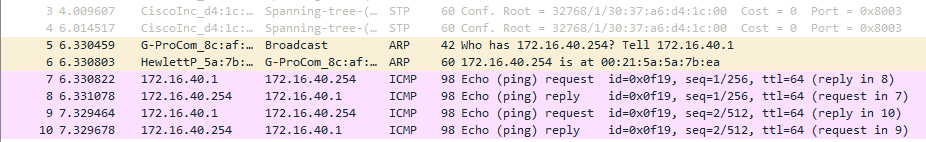
\includegraphics[width=\linewidth]{exp1_wireshark.png}
  	\caption{Experiment 1 - log}
  	\label{fig:Experiment 1 - log}
	\end{center}
	\end{figure}

	\subsubsection{Configuração de duas Redes \textit{LAN} virtuais num \textit{switch}}
	
	\begin{figure}[H]
	\begin{center}
  	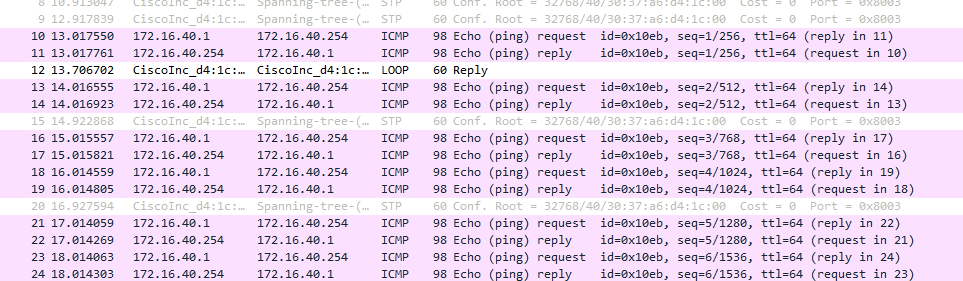
\includegraphics[width=\linewidth]{exp2_6_t2.png}
  	\caption{Experiment 2 - Point 6}
  	\label{fig:Experiment 2 - Point 6}
	\end{center}
	\end{figure}

	\begin{figure}[H]
	\begin{center}
  	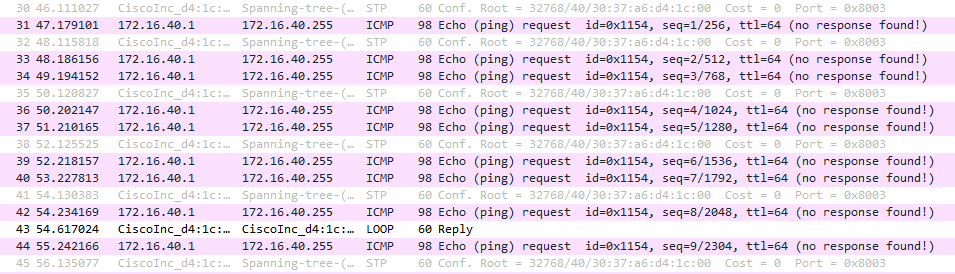
\includegraphics[width=\linewidth]{exp2_9_tux1.png}
  	\caption{Experiment 2 - Point 9 - tux1}
  	\label{fig:Experiment 2 - Point 9 - tux1}
	\end{center}
	\end{figure}

	\begin{figure}[H]
	\begin{center}
  	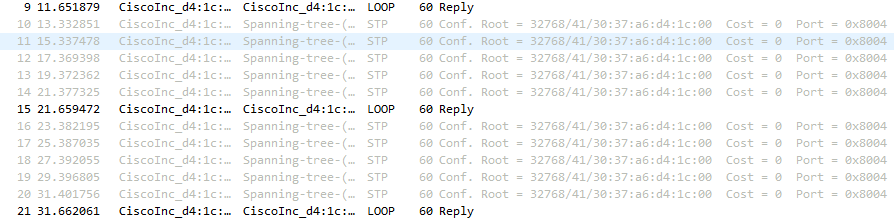
\includegraphics[width=\linewidth]{exp2_9_tux2.png}
  	\caption{Experiment 2 - Point 9 - tux2}
  	\label{fig:Experiment 2 - Point 9 - tux2}
	\end{center}
	\end{figure}

	\begin{figure}[H]
	\begin{center}
  	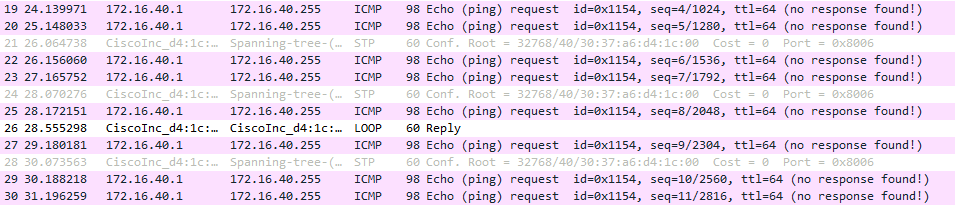
\includegraphics[width=\linewidth]{exp2_9_tux4.png}
  	\caption{Experiment 2 - Point 9 - tux4}
  	\label{fig:Experiment 2 - Point 9 - tux4}
	\end{center}
	\end{figure}

		\begin{figure}[H]
	\begin{center}
  	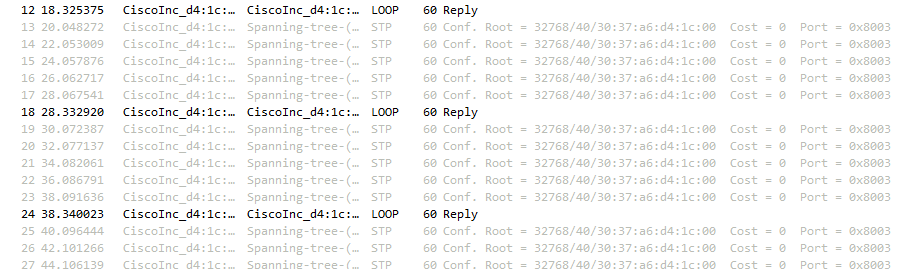
\includegraphics[width=\linewidth]{exp2_10_tux1.png}
  	\caption{Experiment 2 - Point 10 - tux1}
  	\label{fig:Experiment 2 - Point 10 - tux1}
	\end{center}
	\end{figure}

	\begin{figure}[H]
	\begin{center}
  	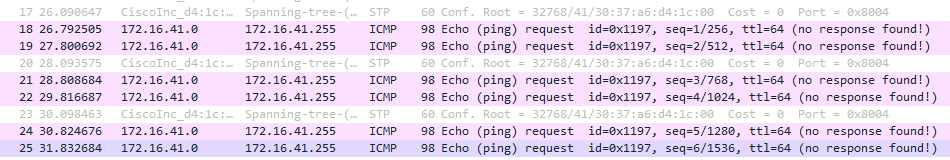
\includegraphics[width=\linewidth]{exp2_10_tux2.png}
  	\caption{Experiment 2 - Point 10 - tux2}
  	\label{fig:Experiment 2 - Point 10 - tux2}
	\end{center}
	\end{figure}

	\begin{figure}[H]
	\begin{center}
  	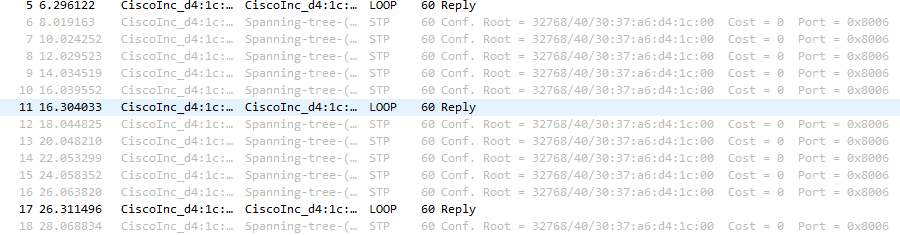
\includegraphics[width=\linewidth]{exp2_10_tux4.png}
  	\caption{Experiment 2 - Point 10 - tux4}
  	\label{fig:Experiment 2 - Point 10 - tux4}
	\end{center}
	\end{figure}

	\subsubsection{Configuração de um \textit{router} em \textit{Linux}}

	\begin{figure}[H]
	\begin{center}
  	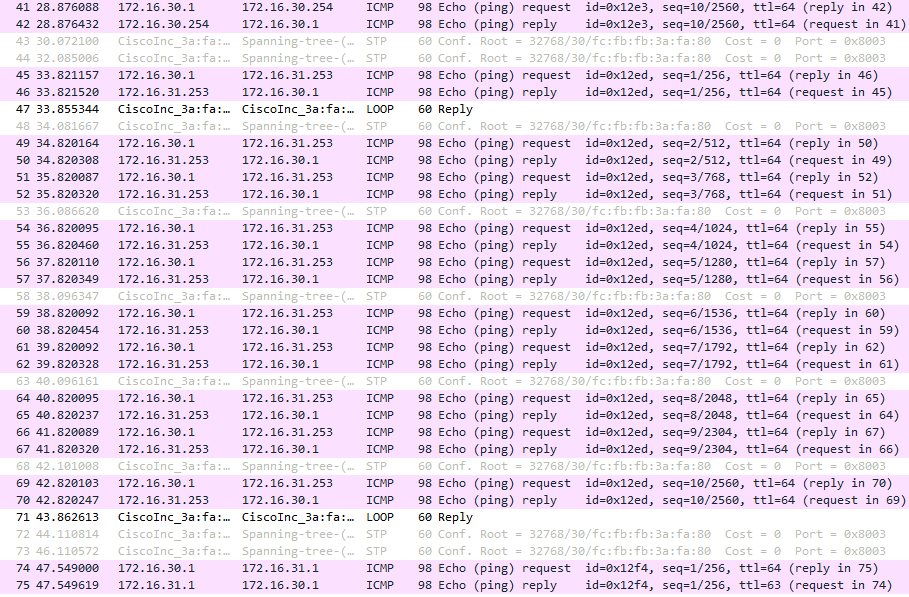
\includegraphics[width=\linewidth]{exp3_tux1.png}
  	\caption{Experiment 3 - tux1}
  	\label{fig:Experiment 3 - tux1}
	\end{center}
	\end{figure}

	\subsubsection{Configuração de um \textit{router} comercial implementando \textit{NAT}}

	\begin{figure}[H]
	\begin{center}
  	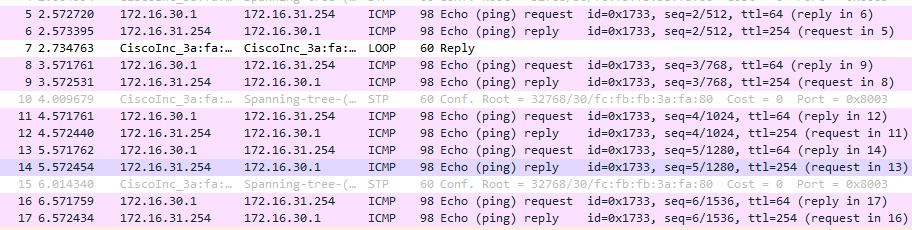
\includegraphics[width=\linewidth]{exp4_tux1.png}
  	\caption{Experiment 4 - tux1}
  	\label{fig:Experiment 4 - tux1}
	\end{center}
	\end{figure}

	\subsubsection{\textit{DNS}}

	\begin{figure}[H]
	\begin{center}
  	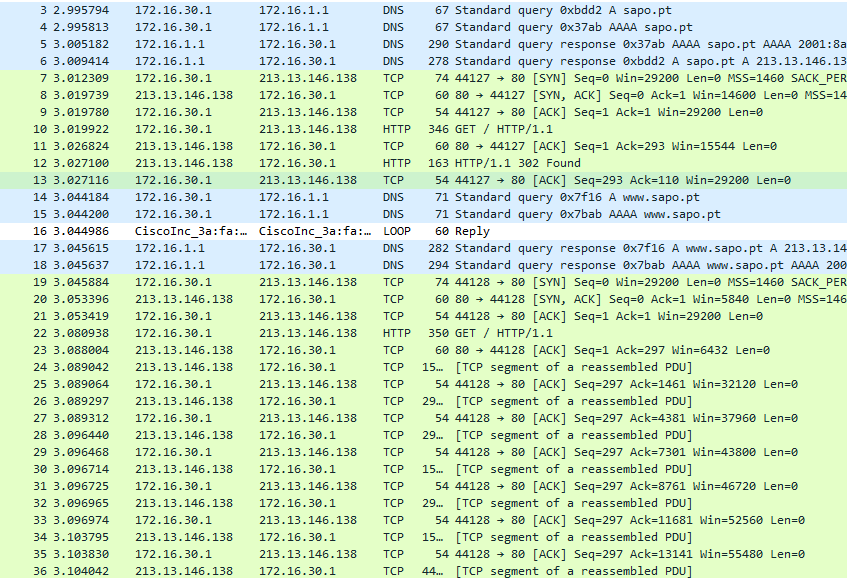
\includegraphics[width=\linewidth]{exp5_tux1.png}
  	\caption{Experiment 5 - tux1}
  	\label{fig:Experiment 5 - tux1}
	\end{center}
	\end{figure}

	\subsubsection{Conexões \textit{TCP}}

	\begin{figure}[H]
	\begin{center}
  	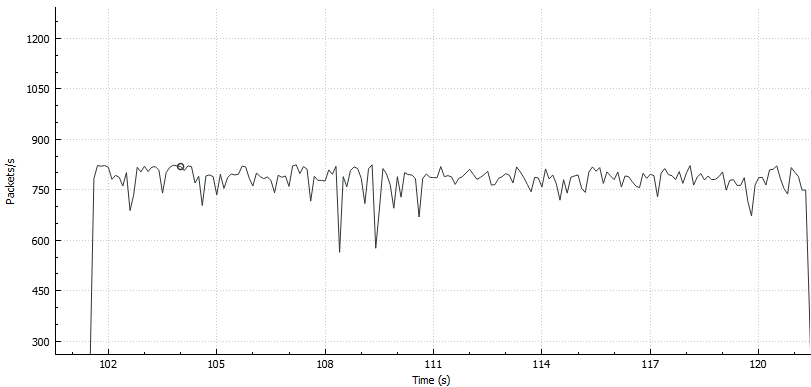
\includegraphics[width=\linewidth]{exp6_tux1.png}
  	\caption{Experiment 6 - tux1}
  	\label{fig:Experiment 6 - tux1}
	\end{center}
	\end{figure}

	\subsection{Application Screenshots}

	\begin{figure}[H]
	\begin{center}
  	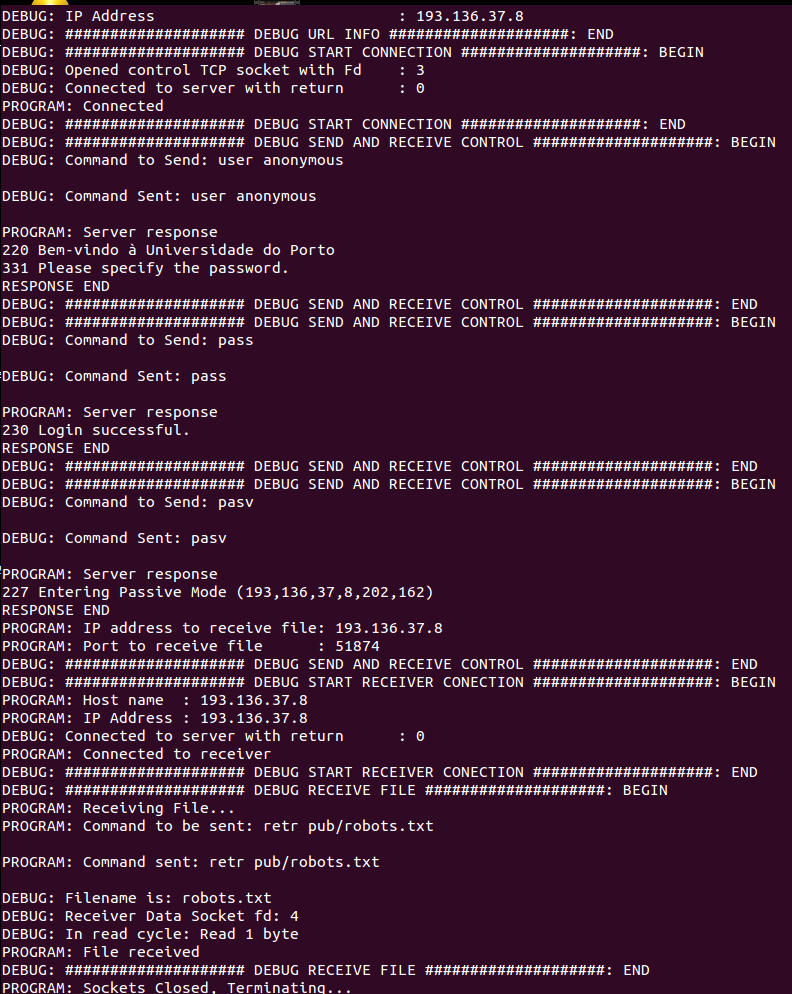
\includegraphics[width=\linewidth]{ftp1.png}
  	\caption{Downloader output - DEBUG mode ON}
  	\label{fig:Downloader output - DEBUG mode ON}
	\end{center}
	\end{figure}

	\begin{figure}[H]
	\begin{center}
  	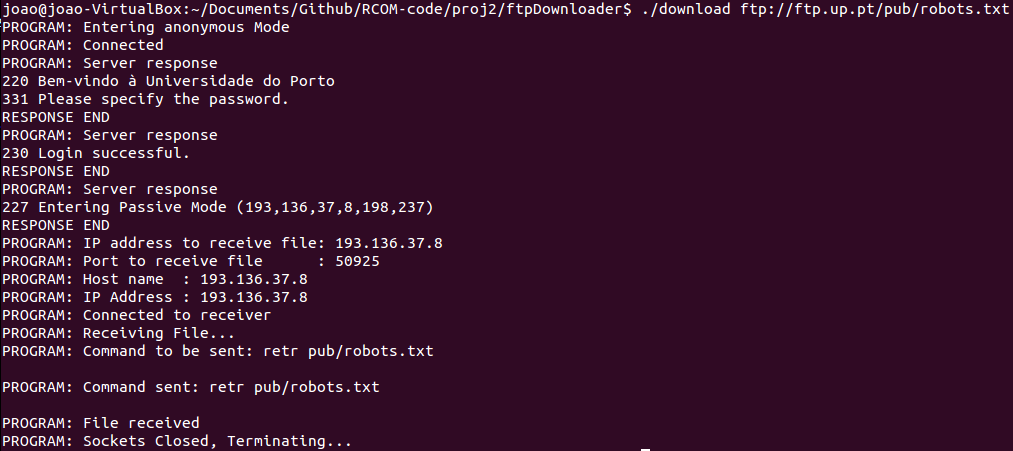
\includegraphics[width=\linewidth]{ftp2.png}
  	\caption{Downloader output - DEBUG mode OFF}
  	\label{fig:Downloader output - DEBUG mode OFF}
	\end{center}
	\end{figure}

	\begin{figure}[H]
	\begin{center}
  	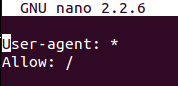
\includegraphics[width=0.2\linewidth]{ftp3.png}
  	\caption{Downloaded file's content}
  	\label{fig:Downloaded file's content}
	\end{center}
	\end{figure}

	\end{document}
